\documentclass[]{article}
\usepackage{fancyhdr}
\usepackage{graphicx}
\usepackage{caption}
\usepackage{abstract}
\usepackage{multicol}
\usepackage{dblfloatfix}
\usepackage{sidecap}
\usepackage{wrapfig}
\usepackage[table,xcdraw]{xcolor}
\graphicspath{ {fig/} }
\usepackage{indentfirst}
\fancyhf{}
\usepackage[margin=1in]{geometry}
\lhead{Program Director/Principal Investigator (Last, First, Middle): Wright, April Marie}
\lfoot{OMB No. 0925-0001/0002 
(Rev. 03/16 Approved Through 10/31/2018) P\thepage.   Continuation Format Page}
\renewcommand{\footrulewidth}{0.4pt}
\pagestyle{fancy}

\begin{document}
\setlength{\headsep}{0.1in}
\setlength{\footskip}{10pt}

\section*{Section 1: Cover Page}
\textbf{Project Title:} ``Modeling Heterogeneous Data Sources for Time-Scaling Phylogenetic Trees`` \\
\textbf{Performance Sites:} Southeastern Louisiana University, Louisiana State University \\
\textbf{Lead Project Investigator:} Dr. April Wright \\
\textbf{Key Personnel:} Mentor Dr. Jeremy Brown, Louisiana State University \\
\textbf{Human Subject Use:} No \\
\textbf{Vertebrate Animal Use:} No \\


\newpage
\section*{Section 2: Abstract and Specific Aims}
Inference of phylogenetic trees is of interest to researchers in many areas of biology.
Phylogenetic trees are used in population-level analyses of evolution and ecology, studies of agriculture, and the study of medicine.
Time-scaling of phylogenetic trees allows researchers to put absolute ages on the nodes in a phylogeny. 
In time-scaling a phylogeny, researchers disentangle the relationship between evolutionary rate and the time since lineages diverged (i.e., an ancestral population became two independent daughter lineages). 
This allows researchers to make a myriad of powerful statements about the rate at which evolutionary change accumulates, how body and genomic features evolve, and how lineages diversify. 
These analyses, while powerful, are also parameter-rich and complex. \par

While researchers are looking to perform increasingly complicated phylogenetic analyses, datasets are also growing larger and more heterogeneous. 
Molecular datasets often encompass many loci, if not whole genomes. 
Time-scaling a phylogeny involves external data sources from which absolute time can be derived. 
This means that researchers are often incorporating fossil data, and other absolute age data (such as geological features) into these analyses, substantially increasing the complexity of the models needed to describe the data. 
As a result, researchers are dealing with more and more data, while simultaneously attempted increasingly parameter-rich methods. \par

Ants (Formicidae) are an excellent system to test if  recent methodological advancements can be used more widely. 
There are large molecular, morphological, and age data resources available. 
Ants display many characteristics analogous to pathogenic evolution, such as periods of rapid lineage accumulation and strong among-lineage variation in their rate of evolution.
It is, therefore, possible to test the predictive ability and analytical capability of new methods for modeling heterogeneous data in this system, and to make recommendations of broader applicability. 

\begin{itemize}
	\item Aim One: Identifying lineage-specific modes of evolution
	\item Aim Two: Evaluating time-stratified evolutionary models for time-scaling phylogenetic trees
	\item Aim Three: Scaling Up An Undergraduate Training Pipeline For Statistical Literacy and Computational Biology

\end{itemize}
\pagebreak

\section*{Section 3: Background and Preliminary Results}
\subsection*{How are phylogenetic trees used in biomedical research?}

\begin{SCfigure}
	
    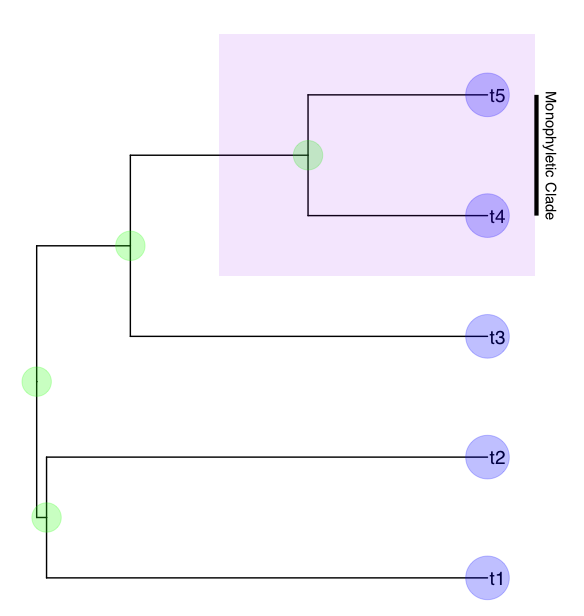
\includegraphics[width=.5\textwidth]{fig/Fig1.png}
       \caption{A graphic displaying a phylogeny. \textbf{Tips}, the taxonomic units we want to know the relationships between are highlighted in blue. \textbf{Nodes}, which represent most recent common ancestors between the lineages that subtend them, are higlighted in green. In the purple box is a \textbf{clade}, which represents a common ancestor and all its descendent lineages (monophyletic).}
\end{SCfigure}

Once the domain of systematic and taxonomic research, phylogenetic trees are found in most areas of biological literature. 
Phylogenetic trees are hypotheses about the relationship between the taxa on them (the tips, see Figure 1).
Tips may be species, they may be higher taxonomic units, or they may be populations or even individuals of interest.
From its earliest beginnings, phylogenetic trees have provided an organizational framework for thinking about biological diversity \cite{hennig1966}. 
As a hypothesis of evolutionary history, phylogenetic trees provide a natural way to classify organisms \cite{de1992} into groupings. 
This type of classification of organisms, often called the phylogenetic species concept, is based on the idea that species should be comprised of lineages on a phylogenetic tree that are independent of any other lineages.
These groupings can then be used to make statements about the evolution of the lineage itself, or the traits that the organisms possess. 
An early example of this type of research in the biomedical community was in the case of Whipple's disease, a gastroenterological disorder.
The bacterium causing the disease was resistant to being cultured in the lab, making characterizing the behavior of the pathogen challenging.
However, amplifying the 16S gene from a tissue sample of a Whipple's patient, and the sequence was placed on a phylogeny with 16S genes isolated from other bacteria.
This allowed researchers to predict, correctly, that the bacteria causing Whipple's disease was gram-positive \cite{relman1992}. \par

Time-scaled phylogenetic trees provide, in addition to a taxonomic framework in which to conduct work, a temporal one.
On a non-time-scaled phylogenetic tree, branch lengths are equivalent to the expected number of substitutions per site; that is, how many base pair changes per site in the molecular sequence data are expected to be observed between a node (a most recent common ancestor) and its descendent (Fig. 1). 
In a tree that has been scaled to time, the branch is equal to the amount of time between a node and a descendent. 
The most common scales for time-scaled phylogenetic trees are millions of years, but for pathogens and other organisms of biomedical interest, the scale may be years or even days.
Uncovering the temporal scale of biological evolution allows researchers to make and test explicit claims about the rate of trait or organismal evolution.
A key example of this type of work is the influenza vaccine.
In choosing the influenza vaccine, a phylogenetic tree is constructed and scaled to absolute time.
This analysis allows researchers to disentangle rate and time - the branches are no longer in expected substitutions per site (a rate), but in time, with rate being a separate parameter.
Since the infectivity of the influenza virus relies on evading the host immune system, strains with a high rate of evolution are of particular interest \cite{timofeeva2017}.
Without the ability to time-scale phylogenetic trees, calculating this information from large scale influenza datasets would be hobbled \cite{paessler2017}.
\par
In recent years, new algorithms to mechanistically model evolution through time in across multiple data sources have been described \cite{stadler2010, heath2014, stadler2017}. 
Called fossilized birth-death models, these mathematical constructs allow researchers to describe the process of evolution that leads to the observed distribution of sequences and phenotypic data at the tips.
These models make explicit assumptions about the process of speciation (addition of lineages), extinction (removal of lineages), and sampling of lineages in the past and the present.
They also present a more straightforward framework for the integration of other data sources, such as fossils or age information.
These models will be discussed in the following paragraphs, but have been readily adopted by the biomedical community as `phylodynamic' models.
For example, phylodynamic models have been used to support hypotheses about the change in populations over time with respect to antigen evolution \cite{Bell432054}.

\subsection*{How have heterogeneous data types been incorporated in phylogenetic analyses?}

Integration of multiple data sources to improve phylogenetic estimation and time scaling of trees has a long history. 
In fact, shortly after the first algorithmic approaches \cite{Farris1970} because available, researchers began to use mutation rate data to establish a time scale of evolution \cite{Zuckerkandl1962, Zuckerkandl1965}. The earliest approaches to this problem are often referred to as `strict' clock approaches, in which the rate of evolution is assumed to be constant across the tree, or all rates are assumed to be drawn from a common distribution of rates specified by the researcher.
While initially quite fruitful, it quickly became clear that variation in organismal life history traits meant that evolutionary rate is not distributed evenly across the tree of life.
To incorporate the variation in evolutionary rate implied by external data sources, models were proposed to allow branches to have different rates of evolution.
These are often called `relaxed clock' models \cite{zheng2001dispersion, Lepage2007}. \par
These models treat time information, whether from fossils, geological information, or sampling dates, as a separate stream of information.
This information is often added to the tree as a node calibration, a value used to constrain the range of possible ages a node can have. 
In practice, performing time-scaling in this way leads to multiple layers of subjectivity being added to the analysis.
First, specimens, such as fossils, must be placed on a branch by an expert.
Secondly, the time between the occurrence of a sample and the node from which it originated must be parameterized, a practice fraught with concerns \cite{Ho2006, heath2014}. 
Lastly, only one constraint can be used per node, forcing researchers to choose a sample, as opposed to using the whole of the data. \par
To alleviate these concerns, the fossilized birth-death model was proposed.
Under the fossilized birth-death model, a phylogeny and its node ages are jointly inferred from all of the available data - nucleotide sequence data, morphological data, and occurrence time data \cite{heath2014}. 
FBD has four parameters: speciation, extinction, past-time sampling of lineages and present-time sampling of lineages \cite{stadler2010}.
This model is fit to the data, and used in conjunction with a model of molecular sequence evolution, and evolutionary rate change to co-estimate the tree and node ages. 
In treating all data as part of the same generating process, the FBD model poses a novel and powerful framework for testing hypotheses about evolution, rates, and time \cite{Stadler2017}. \par

\subsection*{Previous work completed on pilot project to PI Wright}

I was awarded a Louisiana Biomedical Research Network Pilot Project for the 2018-2019 school year.
The project had several major goals: exploring the use of a Dirichlet process prior to improve the efficiency of several phylogenetic computations, and expanding computational training of undergraduates at Southeastern Louisiana University.
In the first four months of funding, several outcomes have been reached.
I have implemented the model proposed in the grant.
I have also trained several students in computational biology, who are now benchmarking the performance of the model.
I currently have an R package in peer review to automate several data processing steps related to phylogenetic computations. \par
In regards to the proposed coursework I suggested in the proposal, I am currently teaching a new course, `Biology 408/508: Computational Biology' for undergraduate and graduate researchers.
I will be teaching a follow-up research course in Spring 2018.
To assist in teaching complex computational concepts to undergraduates, I also developed a web-based tool, treeSiftr, to visualize phylogenetic trees.
A publication for this application is currently being peer-reviewed. \par

\pagebreak
 
\section*{Section 4: Research Plan and Timeline}
\begin{figure}
    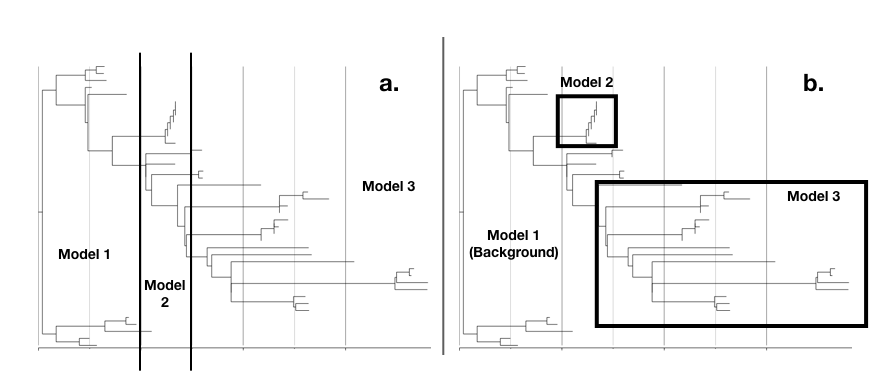
\includegraphics[width=1\textwidth]{2ab}
      \caption{A gaphic demonstrating the two model types. In Fig 1a, the tree is broken up by depth. One FBD process operates deep in the tree, one shallower and one at the shallowest level. In Fig 1b, different lineages on the tree have different FBD models. There is one background model that applies to lineages that do not have a separate process specified.}
  \centering
\end{figure}
\subsection*{Aim One: Time-stratified approaches to divergence time estimation}
The first class of models I would like to examine is the set of `time-stratified models`. 
Under a time-stratified model, the process of evolution is held to change with time.
Biologically, a time-stratified model describes a situation in which some factor of the environment changes with time to be more favorable (leading to higher speciation), or less favorable (leading to higher extinction).
A well-documented example of this type of dynamic is the KT extinction event.
Following the extinction of the dinosaurs, many lineages \cite{brusatte2016, Longrich15253, longrich2012mass} were shown to have greatly increased rates of speciation to fill ecological roles vacated by extinct dinosaurs.
In the study of disease-bearing organisms, this dynamic has also been observed.
For example, large gatherings for the Brazil World Cup facilitated massive transmission of Zika virus \cite{rife2017phylodynamic}.
This short-term event changed the diversification dynamics of the virus by allowing lineages to accumulate rapidly. \par
Ants (Formicidae) have similar dynamics. 
Samples of ants from the fossil record are unevenly distributed. 
As shown on Fig. 3, there are periods with few ant fossils, and periods with a great many, often corresponding to an amber deposit.
These time periods of abundant fossils are well-defined, marked by increased sampling of fossils, and known to biologists.
I would like to test the sensitivity of FBD models by comparing time-stratified FBD models to a time-homogeneous model. \par

\subsubsection*{Implementing and testing models of time-stratified evolution}

To test these time-stratified models, I will use ants (Formicidae).
Ants are a wonderful study system for several reasons.
The first is that there are abundant data for them.
For the dataset, I have 12 nuclear and mitochondrial genes sequenced for 666 species of ants.
I also have a set of 800 fossil occurrences with dates. 
Southeastern Louisiana University does not have pathogen handling facilities, nor do I have training in doing so.
However, the sampling that ants have, as seen on Figure 3, mimics the type of boom-and-bust periods shown by pathogens such as Zika virus \cite{boskova}. 
Therefore, ants form a safe model system in which theories about diversification can be tested. \par

To test if time-stratified models improve the estimation of divergence times, I will first compute a phylogeny from the total set of molecular data and fossil occurrence information using a time-homogeneous FBD model. 
This model assumes that while lineages may have different rates of evolution, the combination of speciation, extinction, and sampling parameters that generated all the fossil and molecular data are invariant with time. 
I will use Stepping Stone sampling \cite{Xie2011} to compute a precise marginal likelihood to the data, so that goodness-of-fit can be compared between this model, time-stratified models, and lineage specific models. \par
Then, I will specify time intervals. 
One model will be a time-homogenous FBD model, for testing purposes.
Two models are derived from the distribution of fossil ages shown on  Figure 3, and visualized in Table 1.
Lastly, I will generate a set of random time intervals, so that the confounding factor of simply adding model parameters can be examined. 
For each model, I will estimate a phylogeny and marginal likelihood. 
I will then use the marginal likelihood to make statements about the goodness-of-fit of each model to the data.
A random set of intervals will allow me to tell if goodness-of-fit is improving because more complex models simply explain more variation, or if the models are picking up on true signal in the data.
Additionally, I will compare the phylogenetic trees and age estimates between the best-fit model and the other models.
This will allow me to make statements about which process of evolution best describes the data, and what the consequences are to not choosing the evolutionary model carefully. \par
\subsubsection*{Expected results}
  \begin{wrapfigure}{left}{0.5\textwidth}
    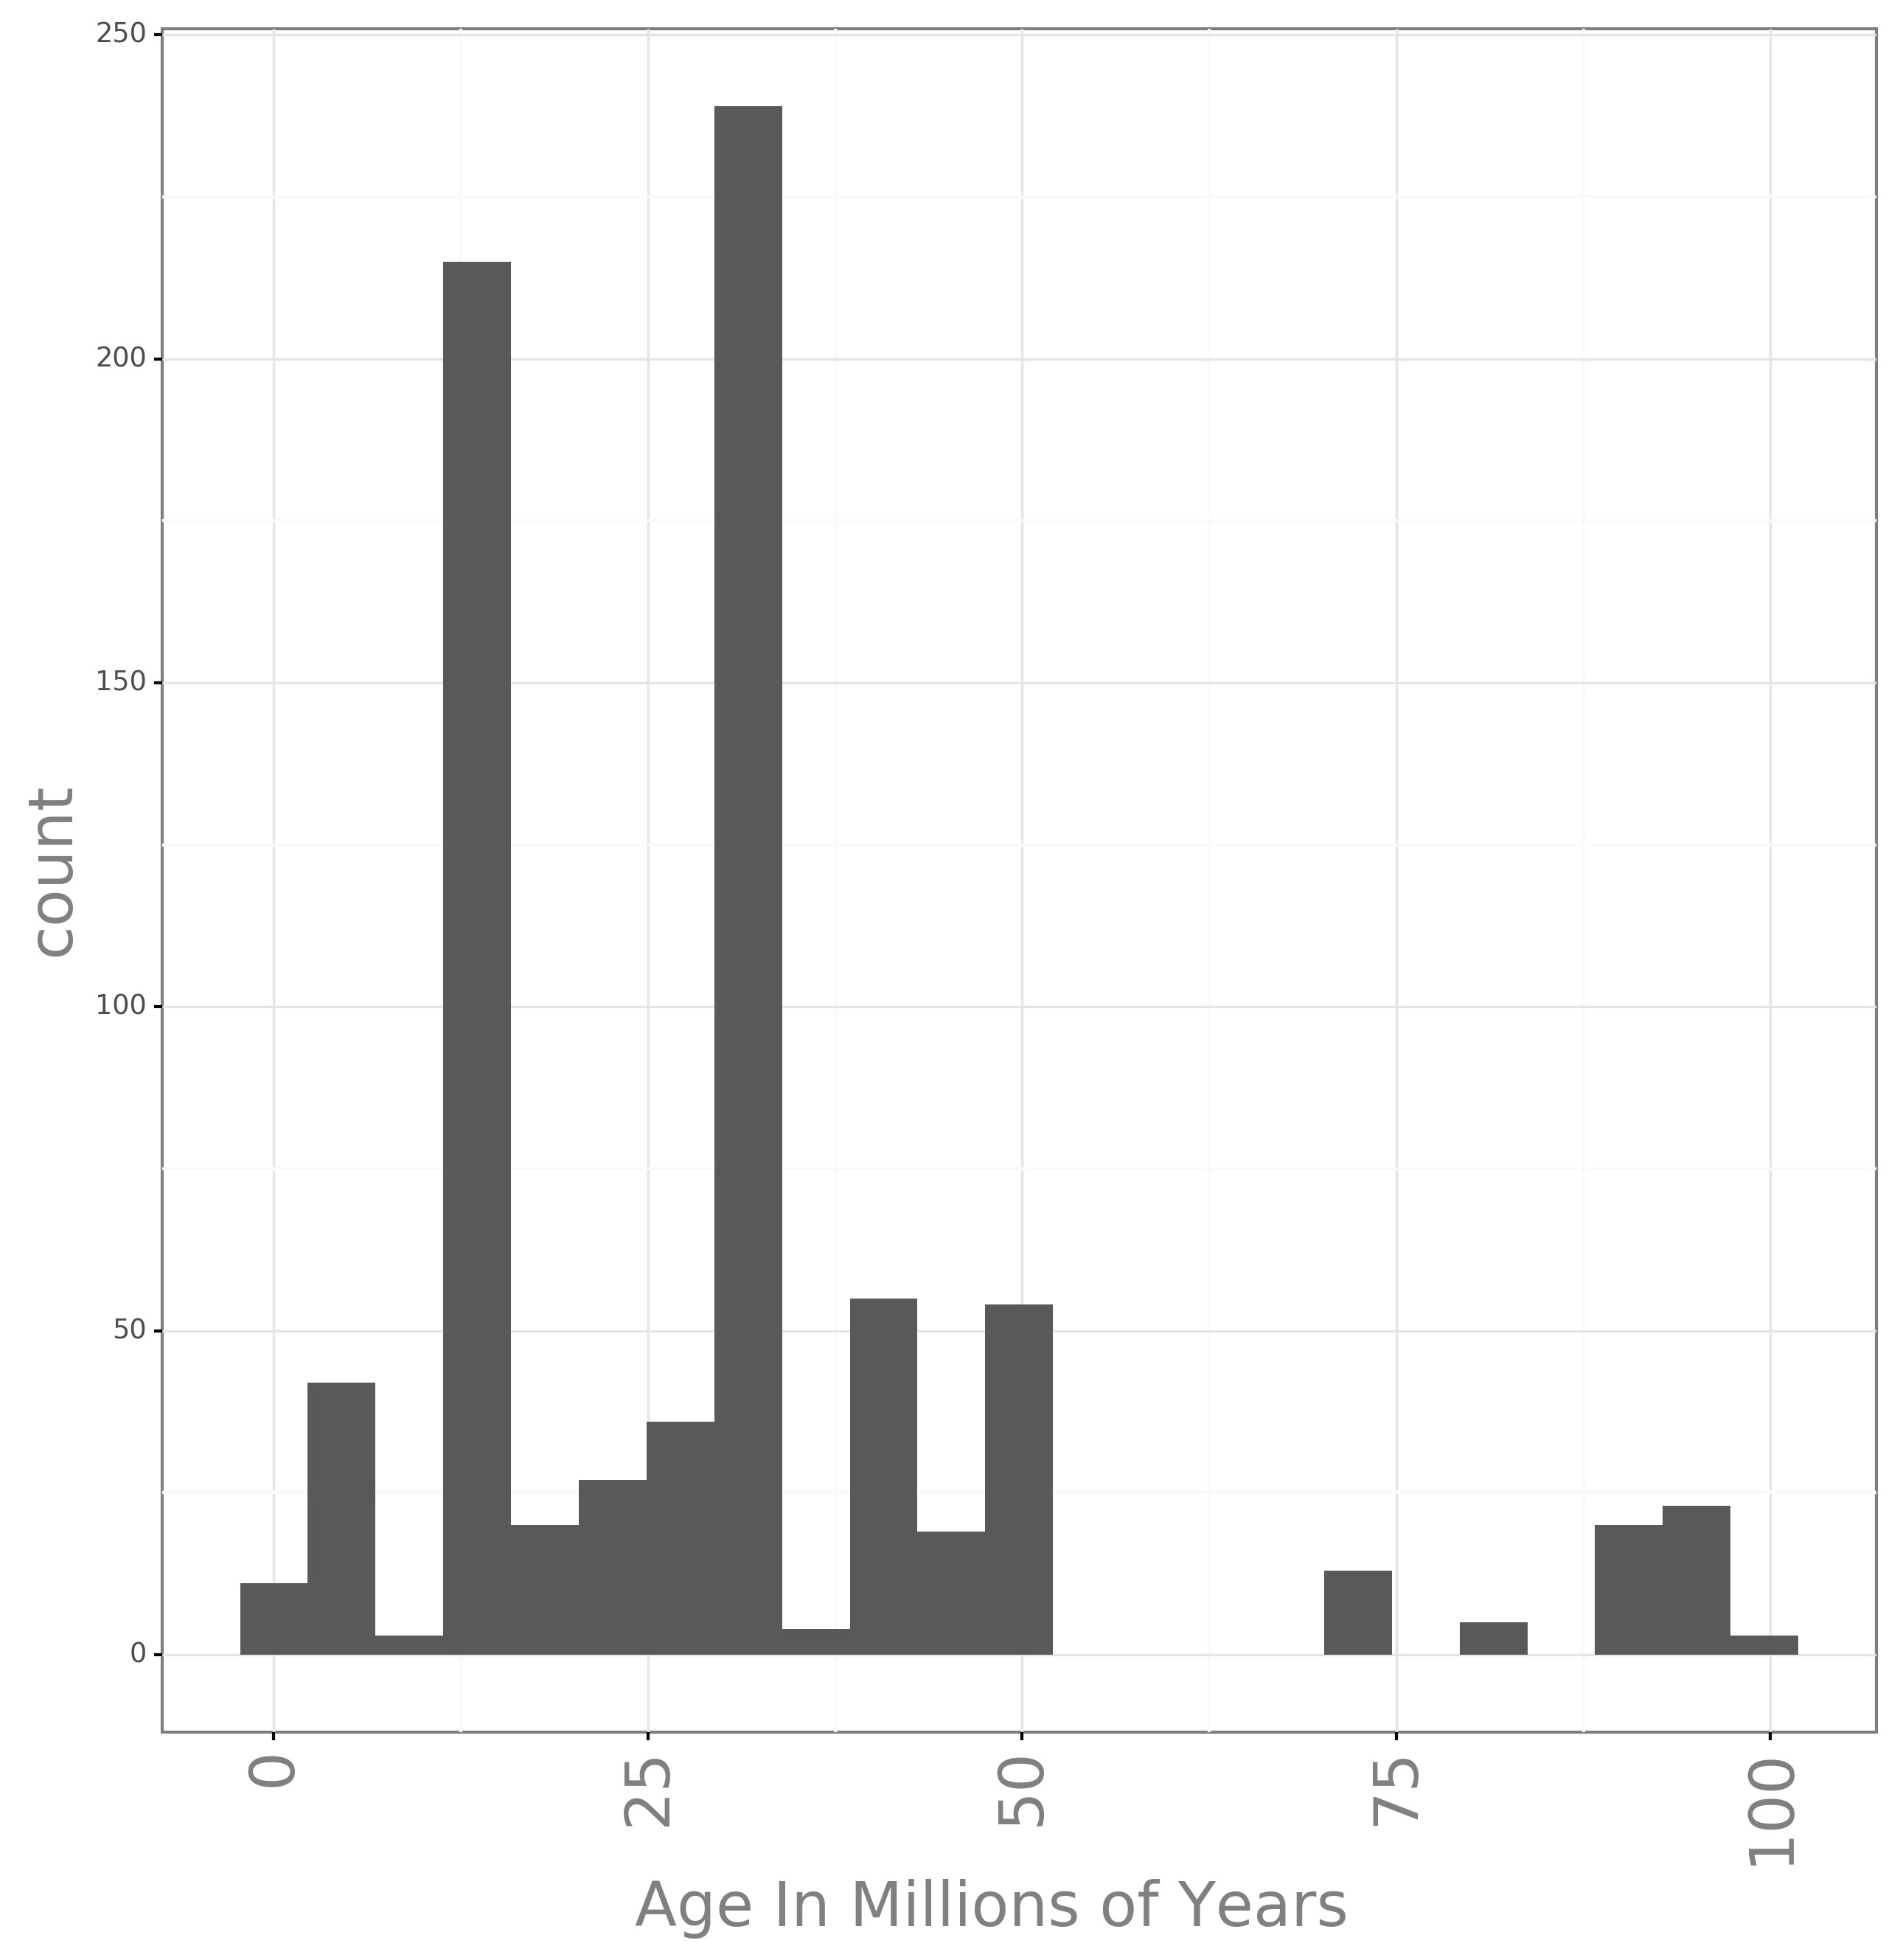
\includegraphics[width=.5\textwidth]{Fig4.png}
     \caption{Number of ant fossil specimens per unit time.}
\end{wrapfigure}
Prior empirical results have indicated that time-stratified models may improve phylogenetic inference \cite{Volz2018}, relative to a time-homogeneous model.
I, therefore, expect that time-heterogeneous models will fit the data better.
However, prior studies have not been working in systems like Formicidae, in which such an abundance of sampling data are available.
Because of this, I expect that the high volume of past-time samples will allow me to estimate a phylogeny and divergence times extremely precisely. \par
\begin{table}[]
\begin{tabular}{l|l|ll}
 & Treatment & Time slices, in millions of years ago &  \\ \cline{1-3}
Scheme One & Time-Homogeneous Model & None &  \\ \cline{1-3}
Scheme Two & Coarse Time-Heterogeneous Model & 4: 0-25, 25-50, 50-75, 75-100 &  \\ \cline{1-3}
Scheme Three & Finer Time-Heterogeneous Model & 5: 0-15, 15-30, 30-50, 55-85, 85-100 &  \\ \cline{1-3}
Random & Random schemes & \begin{tabular}[c]{@{}l@{}}Generate distributions of 4 and 5 \\ scheme models for comparison\end{tabular} & 
\end{tabular}
    \caption{Model specification schemes for the research described in Aim One.}
    \end{table}


\subsection*{Aim Two: Specifying lineage-specific models of evolutionary process}

Variation among lineages in evolutionary tempo initially spurred development of methods to accommodate different rates of evolution on a phylogeny.
These methods, discussed above as relaxed clock models, have been a boon for researchers working with all types of data.
For example, relaxed clock methods continue to be used in molecular characterization and analyses of HIV \cite{park2016}. 
Non-microbial organisms also show strong signatures of among-lineage rate variation \cite{bapst2016}. \par
However, these methods incompletely incorporate occurrence time information, which can lead to biases in date estimates \cite{heath2014, slater214}.
It has also been demonstrated that failing to account for evolutionary mode can generate misleading age and rate estimates. 
Therefore, I would like to explore the use of models that allow not simply the evolutionary rate, but the parameters of the FBD analysis to vary.
Speciation, extinction, and sampling parameters control the fundamental shape of the tree. 
If one lineage has a very high speciation rate, it will accumulate many more lineages than one with a lower rate of evolution.
Co-estimating the rates of speciation and extinction alongside the tree and the rates of evolution will give us both finer-scale resolution on node ages, as well as a testable framework for locating lineages to make predictions about the evolutionary process. \par
The approach of allowing time-stratified evolutionary processes has already been shown to be effective in many study systems, as discussed in the section whatever.
However, it is not expected that variation is time-stratified in all lineages.
For example, among-lineage rate variation is suspected to be a driver of differences in viral replication among influenza B viruses \cite{timofeeva2017}.
Southeastern is not set up for pathogen handling, however, the ant dataset is well-suited to the study of this particular question.
Ants have known life history variation in where ants live and are sampled.
Extinct ants that lived in trees are more likely to be sampled, because they are preserved in amber.
Extinct ants with a ground habit are less likely to be sampled, due to poor preservation. 
Therefore, different lineages of ants are expected to be evolving according to different, lineage-related, evolutionary models. 
This is visualized Fig 2b. \par

\subsubsection*{Implementing and testing models of lineage-specific evolution}
  \begin{wrapfigure}{left}{0.5\textwidth}
    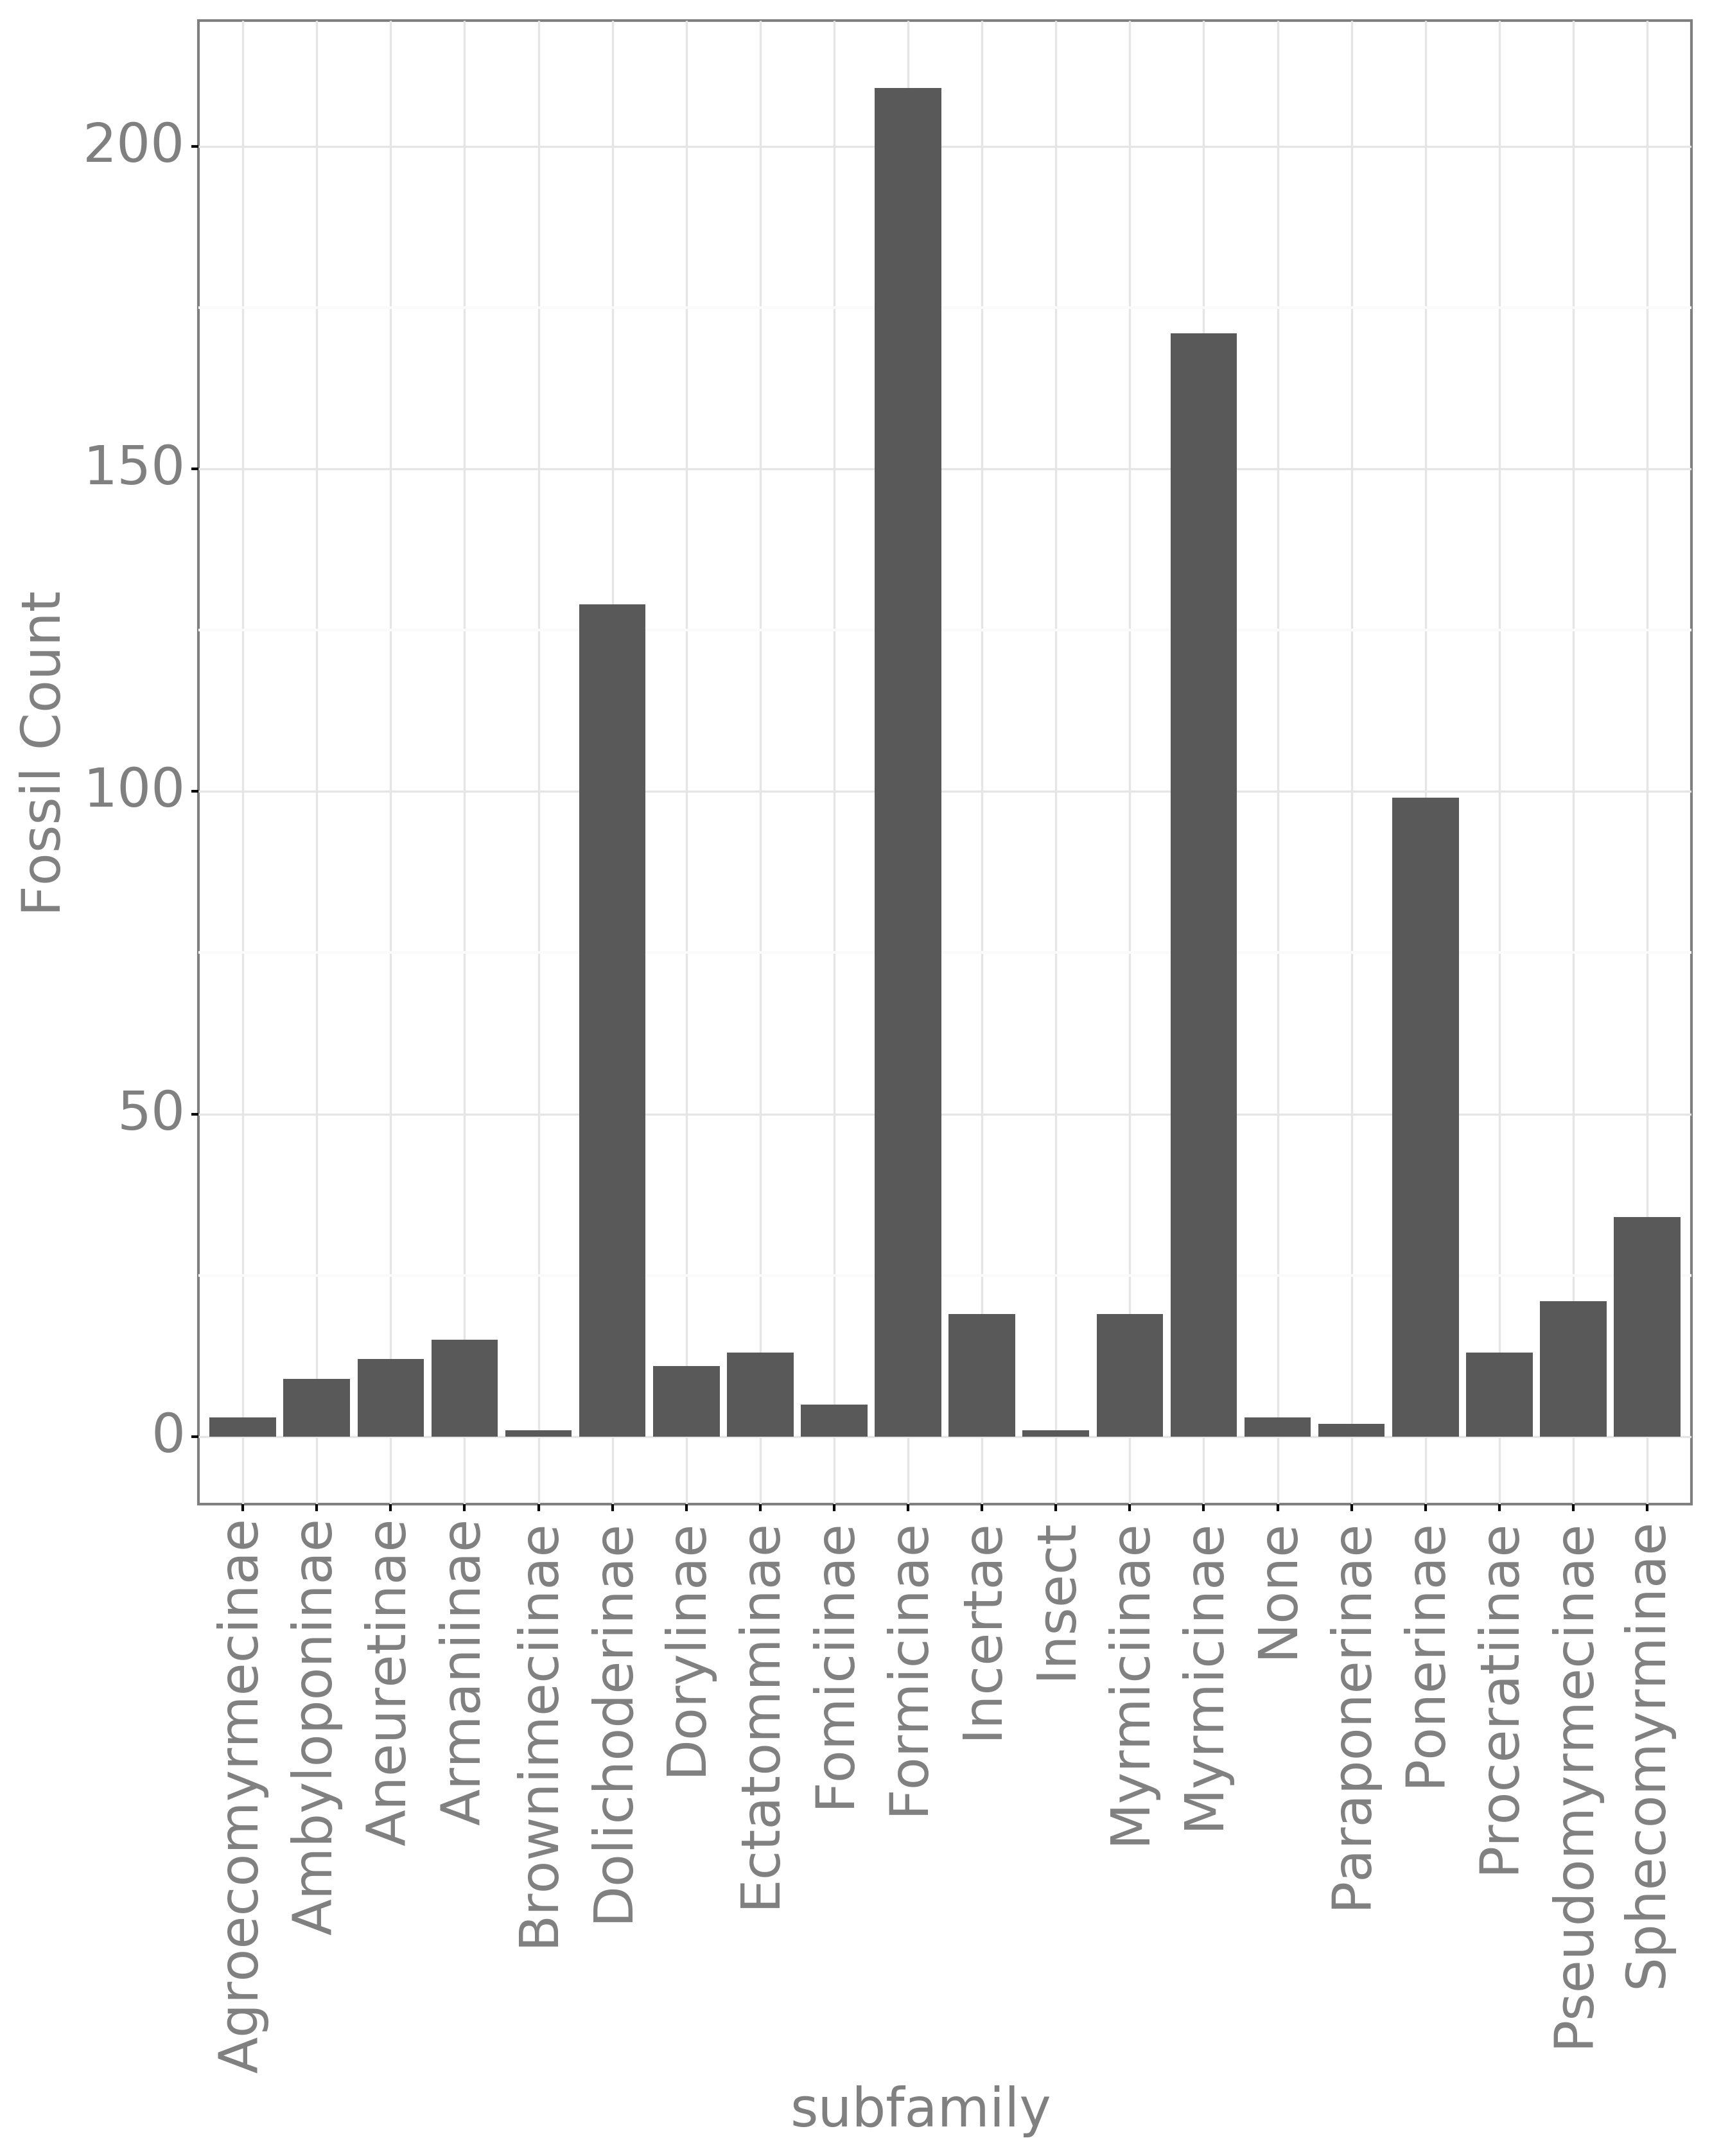
\includegraphics[width=.5\textwidth]{Fig3.png}
     \caption{Number of ant fossil specimens per subfamily.}
\end{wrapfigure}
Lineage-specific FBD models have not yet been published, or extensively tested.
There is an implementation of this model in the software RevBayes.
I will use this implementation to perform a series of model-fitting comparisons. 
The Formicidae has 21 subfamilies.
At least 15 of these groups have fossil information.
The number of fossils per group is visualized on Figure 3.
Because these are fossils, the type of fossil can be taken as a proxy for life history.
Therefore, I can divide the tree into separate regions based on the expected evolutionary model.
For example, the ants known primarily from amber fossils will be expected to have larger sampling parameters because ants are more likely to be preserved in amber than in the ground. \par
I will, therefore, use an iterative model-fitting approach to test if lineage-specific models of evolutionary variation are sensitive enough to pick up among-lineage variation in a single parameter.
First, I will allow each clade of tree-dwelling ants to have its own evolutionary process, and independent sampling rate.
Secondly, I will combine groups of tree-dwelling ants into a single rate class, such as to furnish a simpler model from which the results can be compared. 
Each model will be have a precise marginal likelihood calculated via Stepping stone model fitting. \par
Once all the models are computed, they will be compared.
Each of the models will be compared to the time- and lineage-homogeneous model computed as part of Aim One.
If a model of lineage-specific evolution has a better marginal likelihood score than the homogeneous model, it will be compared against both the time-stratified models, and the other lineage-specific model. \par
\subsubsection*{Expected results}
By producing this set of comparisons, I will be able to test if these models are sensitive enough to pick up on among-lineage variation in evolutionary process, and I will be able to tell if among-lineage variation or time-stratified variation are more important in this group.
My expectation is that, since we have detailed information about the ecology of ants, that incorporating this information will improve model fit for our phylogenetic estimations.
Since among-lineage rate variation is expected in many groups, including those of biomedical importance, I expect that improving the ability of researchers to incorporate knowledge about the life history of their organisms into phylogenetic and phylodynamic researchers will be an important contribution to the literature.\par

\subsection*{Aim Three: Scaling a Training Pipeline for Statistical and Computational Biology Literacy}

	\subsubsection*{Notebook-Based Coursework For Undergraduate Students}
In my first year, I have greatly expanded the catalog of computational biology courses.
I have taught three computational biology courses, GBIO 690 (Systematics Lab), GBIO 450 (Genomics and Transcriptomics), and GBIO 408/508 (Computational Biology). 
A consistent theme in these courses is students lacking reasonable computers, and Southeastern lacking reasonable computer lab space to house computational courses. 
The majority of students at Southeastern work more than 20 hours a week outside school, and the school serves many armed forces reservists.
Therefore, coursework may be completed on a computer that is not the student's own computer.
I aim to expand my use of technologies that do not require installs on a student or school machine.
\par
In the first iteration of my Computational Biology course, I piloted
the use of JupyterHubs to teach biologists how to analyze data in the Python programming language.
A JupyterHub is a Python server that can be connected to a web-based login portal.
When students arrive in class, they navigate to a course webpage, click a link, and the days' class materials are automatically synced to their home directory on a server for them.
They can then do the day's activities, homework, and labs.
The benefit of this technology is that I do not have to perform installs on Southeastern's laboratory machines, which are rapidly aging.
The students do not have to perform installs, and can do their homework from anywhere, including if they do not have access to their personal computer.
I will be using this technology to teach smaller-scale data visualization in the R programming language in a new course I am offering this spring, Museum Studies. 
This course is a research experience for undergraduates; they will be paired with a graduate mentor who is performing research in the museum.
They will help the student collect data, and then will use R to clean, analyze, and plot their data to make figures for a poster presentation. \par
I am requesting funds to expand the availability of notebook-based coursework.
I experienced significant issues serving courses in Genomics and Transcriptomic and Systematics Lab, predominantly related to students lacking reasonable personal computers.
Converting these courses to a notebook-based framework would solve these issues.
Particularly, I would like to host a sprint at the Scientific Python meetings.
Sprints are designed to bring together like-minded people who are facing similar challenges to work together.
During the sprint, we would develop a set of materials for genomics, phylogenetics, and evolution.
These notebooks would be aimed at upper-division undergraduates who have used Python programming before.  
These materials would be developed on GitHub, and hosted via ReadTheDocs, a popular website for hosting educational materials. \par
During fall 2018, I have been purchasing hosting for my computational biology course's JupyterHub.
The State of Louisiana already has a high-performance cluster computer, the Louisiana Optical Network Infrastructure machines, which will soon be capable of hosting a JupyterHub.
I will work with the staff at LONI to make my materials available as a module that can be loaded by any user of the state compute resources.
This way, instructors can both make use of the compute environment, and the materials, without being located on the Southeastern campus. \par

\subsubsection*{Developing cross-discipline computational training for undergraduates}
\begin{table}[]
\begin{tabular}{l|l|ll}
Section              & Motivating Questions                                                                                                                                                                                                                   & Computational Activity                                                                                                                                                                                      &  \\ \cline{1-3}
Numerical Literacy   & \begin{tabular}[c]{@{}l@{}}``How many cells are in the body?"\\ \\ ``How many generations of humans \\ have there been?"\\ \\ ``How many chemical compounds does \\ a person ingest in a day?"\end{tabular}                            & \begin{tabular}[c]{@{}l@{}}Visualizing different quantities\\ \\ Visualizing the strength of natural \\ selection and genetic drift\end{tabular}                                                            &  \\ \cline{1-3}
Statistical Literacy & \begin{tabular}[c]{@{}l@{}}``What is average? Am I average?"\\ \\ ``How can a machine tell me who is more likely \\ to get cancer?"\\ \\ ``I read on the news that eggs will kill me. \\ Will they?"\end{tabular}                      & \begin{tabular}[c]{@{}l@{}}Plotting basic distributions, and \\ understanding variance\\ \\ Use of mixture models to understand \\ structure in a population\\ \\ \\ Calculating relative risk\end{tabular} &  \\ \cline{1-3}
Biological literacy  & \begin{tabular}[c]{@{}l@{}}``It's Natural - that means it's good, right?"\\ \\ ``We're humans; are humans are very different \\ than animals?" \\ \\ ``My father has high blood pressure, does that \\ mean I will, too?"\end{tabular} & \begin{tabular}[c]{@{}l@{}}Using databases to look up compounds\\ \\ \\ Reading and understanding \\ phylogenetic trees\\ \\ Predicting genotype and phenotype ratios\end{tabular}                          & 
\end{tabular}
    \caption{Course components for an undergraduate, non-majors biomedical literacy course.}
\end{table}
Basic scientific, numerical, and biomedical literacy is a challenge in public life. 
To increase literacy about how computational algorithms shape our understanding of the natural world, I would like to develop a course called `Biomedical Literacy for Everybody'. 
This course will be a course for non-biology majors organized around several core concepts: numerical literacy, statistical literacy, and biological literacy.
These core concepts and example motivating questions are shown on Table 2. \par

It is not reasonable to expect non-science majors to learn to program while learning statistics and biology in one semester.
Therefore, I would like to develop a set of R Shiny applications to allow for hands-on computational inquiry. 
A Shiny application allows an expert to write R functions to perform analyses.
Then, the expert can generate a user-interface that can be hosted and served over the web.
Therefore, students get the experience of working with mathematical functions, while in the familiar realm of point-and-click interfaces.
The custom functions will be developed are noted on Table 2. \par

\section*{Section 4c: Project Timeline}
\begin{table*}[!b]
\begin{tabular}{|l|l|l|l|l|l|l|}
\hline
 & Summer `19 & \begin{tabular}[c]{@{}l@{}}School year \\ `19-`20\end{tabular} & Summer `20 & \begin{tabular}[c]{@{}l@{}}School year \\ `20-`21\end{tabular} & Summer `21 & \begin{tabular}[c]{@{}l@{}}School year \\ `21-`22\end{tabular} \\ \hline
Aim One Research & \cellcolor[HTML]{9B9B9B} & \cellcolor[HTML]{9B9B9B} & \cellcolor[HTML]{9B9B9B} &  &  &  \\ \hline
Aim One Writing &  &  & \cellcolor[HTML]{FFFFFF} & \cellcolor[HTML]{9B9B9B} &  &  \\ \hline
Aim Two Research &  &  & \cellcolor[HTML]{9B9B9B} & \cellcolor[HTML]{9B9B9B} & \cellcolor[HTML]{9B9B9B} & \cellcolor[HTML]{9B9B9B} \\ \hline
Aim Two Writing &  &  &  & \cellcolor[HTML]{FFFFFF} &  & \cellcolor[HTML]{9B9B9B} \\ \hline
Aim Three Development & \cellcolor[HTML]{9B9B9B} &  & \cellcolor[HTML]{9B9B9B} &  & \cellcolor[HTML]{9B9B9B} &  \\ \hline
Aim Three Teaching &  & \cellcolor[HTML]{9B9B9B} &  & \cellcolor[HTML]{9B9B9B} &  & \cellcolor[HTML]{9B9B9B} \\ \hline
\end{tabular}
\end{table*}
\pagebreak

\bibliographystyle{plain}
\bibliography{refs}

\pagebreak

\section*{Section 5: Investigators}
\subsection*{Section 5ai: The Principal Investigator}

I received my PhD from the University of Texas at Austin in 2015. 
I was awarded a National Science Foundation Postdoctoral Research Fellowship in 2016 for work developing and testing models for phylogenetic inference.
Following the fellowship, I joined the faculty at Southeaster in fall of 2017 as an assistant professor. \par
I have experience with software implementations of phylogenetic models.
As a postdoctoral researcher and a new faculty member, I also have a record of training undergraduate students in statistical and computational approaches to the biological sciences. 
I will be involved both in training the students, and in the day-to-day work of the project.
\subsubsection*{Section 5aii: Individual Development Plan}

My goal is to get tenure and develop a sustainable research program.
This funding will assist me in doing that by allowing me to support students, and obtain additional release time to focus on research.
Publication of scientific papers is a requirement of tenure, and this funding will make that possible.
Additionally, National Science Foundation and NIH grants rate broader impacts highly in grant proposals.
Developing a tight relationship between my research and my training activities will make me more competitive for further national funds, which will, in turn, allow me to publish more and devote more time to performing research. \par

\subsection*{Section 5b: The Mentor}

Dr. Jeremy Brown is an associate professor at Louisiana State University.
He joined the faculty at LSU in 2011, after completing a postdoctoral fellowship at the University of California, Berkeley and a PhD at the University of Texas at Austin.
Dr. Brown has a long history of working with cutting-edge approaches to large phylogenetic datasets, as well as statistical approaches for model selection. \par
Dr. Brown also has mentored many graduate and undergraduate students in computational biology.
He is also very involved in other aspects of scientific community service, such as teaching at workshops and serving on councils in his professional society.
Dr. Brown is not requesting support on this proposal.

\subsection*{Section 5c: Undergraduate Research Assistants}

I have identified three promising undergraduates to carry out the work on this proposal. 
These three students are currently being trained on basic methods for computational biology, such as Python programming and high-performance cluster computer use.
The students will be directly involved in vetting training materials, setting up and running phylogenetic estimations, and visualizing results. \par
During the school year, they will receive course credit for participation in the project.
Over the summer, the students will work 40 hours a week on the project. \par





\end{document}